
\begin{dialog}{咏叹调及其种种变奏}

\begin{quote}
这几天阿基里斯夜里一直无法入睡。今晚他的朋友乌龟来了,要陪他度过这烦人的时光。
\end{quote}

\begin{dialogue}

\item[乌龟]亲爱的阿基,听说失眠弄得你很苦恼,我真难过。我希望我来陪伴你能让你放松下来,摆脱那些使你没法入睡的讨厌刺激。也许我会让你烦得不得了,烦得你最后终于睡着了。要是这样,我也算对你有所帮助了。

\item[阿基里斯]噢,不,恐怕到现在我已经见过世界上最出色的烦人能手了,他们都想要让我烦得睡过去——可是真不幸,结果都没什么用。你不会比他们更有办法的。别这么想了,龟兄,我邀你来是希望能扯点儿数论里的玩艺儿消遣消遣,这样我至少可以比较愉快地捱过这漫长的时光。你知道吗,我发现谈点儿数论对我这骚乱的精神大有好处。

\item[乌龟]真是个有趣的怪念头!这让我想起——嗨,是有点像——那个可怜的凯瑟林侯爵。

\item[阿基里斯]他是谁呀?

\item[乌龟]哦,他是十八世纪时萨克森的一位侯爵——老实说,是一位后知后觉的侯爵——可就是因为他——哎,要我讲下去吗?这是个挺有趣的故事呢。

\item[阿基里斯]那还用说,讲下去吧。

\item[乌龟]有一段时期这位好侯爵患了失眠症,很是痛苦。恰巧有个不错的音乐家住在同一个镇上。于是他委托这位音乐家谱写了一系列变奏曲,由侯爵的宫廷羽管键琴师在他的不眠之夜里为他演奏,以便愉快地消磨这些时间。

\item[阿基里斯]那个当地的音乐家能胜任吗?

\item[乌龟]我想他胜任了,因为曲子谱好以后,侯爵非常慷慨地回报了他——侯爵赠给他一只金质高脚杯,里面有一百枚金币。

\item[阿基里斯]真的吗?我首先得知道他哪儿来的那么个高脚杯,还有那些金币。

\item[乌龟]可能是他在博物馆里看见的,然后做了些手脚。

\item[阿基里斯]你是不是暗示说他把它们弄到手后溜走了?

\item[乌龟]好了好了,我不想那么说,不过……那种时候,侯爵是能弄走好多东西的,无论如何,有一点很清楚:那些音乐给侯爵带来了巨大的快乐。因为他不断请求他的羽管键琴师——那时还只是个小伙子,叫哥德堡——为他演奏那三十首变奏曲中的曲子。结果(这多少带点讽刺)那些变奏曲倒和那位年轻人的名字“哥德堡”联系在一起了,而不是跟那位著名的侯爵。

\item[阿斯里斯]你是说,那位作曲家是巴赫,而那音乐就是所谓的《哥德堡变奏曲》?

\item[乌龟]正是!实际上,这部作品取名为《咏叹调及其种种变奏》,一共有三十首。你知道巴赫是怎么把这三十首辉煌的变奏曲组织在一起的吗?

\item[阿基里斯]你告诉我吧。

\item[乌龟]所有曲子——除了最后一首——都基于一个单一的主题,他称之为“咏叹调”。实际上,把曲子结合在一起的不是一支共同的旋律,而是一个共同的和声基础。旋律可以变化,但背后那个主题是稳定的。只是在最后一支变奏曲里巴赫变得随便起来。那是种“终了后的终了”,包含有与原主题几乎无关的多余的音乐——事实上,那是两支德国民歌。那支变奏曲称为“拼凑曲”。

\item[阿基里斯]《哥德堡变奏曲》还有什么不同寻常的地方吗?

\item[乌龟]有。每隔两支变奏曲有一首卡农。第一首卡农中两个轮唱着的声部在同一个音符上加入。在第二首中,轮唱着的声部中的一个加入时比另一个高一个音符。在第三首中,一个声部比另一个声部高两个音符加入。如此类推,直到最后一首卡农加入,恰好相差九个音程。一共十首卡农。而——

\item[阿基里斯]等一下。我好像记起来在什么地方读到过最近新发现了十四首哥德堡卡农……

\item[乌龟]是不是那份刊物上还说最近发现十一月一共有四十四天,其中新添的那十四天以前不为人们所知?

\item[阿基里斯]没错儿。一个名叫沃尔夫的人——一位音乐学家——听说在斯特拉斯堡有一份特殊的《哥德堡变奏曲》副本,就到那里看了看。令人吃惊的是,在纸的背面。作为一种“终了后的终了”,他发现了这十四首新卡农。它们全都基于《哥德堡变奏曲》主题的前八个音符。所以现在大家都知道《哥德堡变奏曲》中的变奏曲一共有四十四首,而不是三十首。

\item[乌龟]也就是说,在另外的什么音乐学家在什么其他鬼地方再发现另一些变奏曲之前,共有四十四首。尽管这看起来不大可能,但也说不定,即便是几乎肯定不会了,也还是有可能会有另一些曲子被发现,然后又发现一些,然后又发现又发现又发现……喔,恐怕这是没个头的!我们大概永远不会知道是否——或何时——我们能得到全部的《哥德堡变奏曲》。

\item[阿基里斯]这倒是个奇怪的想法。大概,每个人都认为这一最新发现仅只是个偶然现象,而我们现在确实真地得到了所有的《哥德堡变奏曲》。不过还是假定你对吧,什么时候也许又会出现一些新的变奏曲。我们可以抱有这种指望。这样的话,“《哥德堡变奏曲》”这个名字的含义就会稍稍有所变化,不仅要包括已经知道的曲子,还要包括任何其他最终会出现的曲子。总数——称之为“$g$”吧——肯定是有限的,你同意吧?——可仅仅知道$g$是有限的并不等于知道$g$有多大。因此,这一信息无法使我们得知什么时候我们能确定最后一支《哥德堡变奏曲》。

\item[乌龟]说的一点不错。

\item[阿基里斯]告诉我——巴赫是什么时候写下这些著名变奏曲的?

\item[乌龟]这是1742年的事,那时他在莱比锡当“康托尔”[Cantor]——就是教堂圣咏班的指挥。

\item[阿基里斯]$1742$?嗯……这个数让人想起什么。

\item[乌龟]理当如此,因为这恰巧是个很有意思的数,它是两个奇素数的和:$1723$与$19$。

\item[阿基里斯]天哪!多么奇特的事情!那么,碰见具有这种性质的偶数的频率会是多少呢?让我们来看看……
\begin{align*}
   6 & =3+3 \\
   8 & =3+5 \\
  10 & =3+7=5+5 \\
  12 & =5+7 \\
  14 & =3+11=7+7 \\
  16 & =3+13=5+11 \\
  18 & =5+13=7+11 \\
  20 & =3+17=7+13 \\
  22 & =3+19=5+17=11+11 \\
  24 & =5+19=7+17=11+13 \\
  26 & =3+23=7+19=13+13 \\
  28 & =5+23=11+17 \\
  30 & =7+23=11+19=13+17
\end{align*}

哦,瞧——按我的这一小张表,似乎这是个很常见的现象。可我到现在也还没看出这张表里有什么显见的规律。

\item[乌龟]也许就没有什么能找得出的规律。

\item[阿基里斯]当然得有!我只不过是不够聪明,现在还看不出来。

\item[乌龟]你好像非常肯定。

\item[阿基里斯]在我看来这是毫无疑问的。我想……会不会所有的偶数(除去$4$)都能写成两个奇素数之和?

\item[乌龟]嗯……这问题让人想起什么……啊,我知道了!你不是第一个问这个问题的人。嗯,事实上,1742年就有个业余数学家提出了这个问题,是在——

\item[阿基里斯]你说的是1742年吗?请原谅我打断你,不过我注意到$1742$恰巧是个很有意思的数,它是两个奇素数的差:$1747$与$5$。

\item[乌龟]天哪!多么奇特的事情!那么,碰见具有这种性质的偶数的频率会是多少呢?

\item[阿基里斯]我还是别让你分心吧,请接着讲你的故事。

\item[乌龟]哦,对——我刚才说到,1742年有个业余数学家——他的名字我一下子记不起来了——寄了封信给欧拉。欧拉那时正在波茨坦腓德烈大帝的宫廷里,于是——哎,要我讲下去吗?这可不是个没劲的故事。

\item[阿基里斯]那还用说,讲下去吧。

\item[乌龟]很好。在信里,这位业余的数论爱好者向伟大的欧拉提出了一个未证明的猜想:“每个偶数都能表示成两个奇素数之和。”这家伙的名字是什么来着?

\item[阿基里斯]我有点想起这个故事了,是在一本什么数论书里。他的名字是不是“席勒艾舍尔”?

\item[乌龟]嗯……不太像,看来不是。那名字就在我的舌尖上——是——是——啊对了!是“哥德巴赫”!这家伙是哥德巴赫。

\item[阿基里斯]我就知道是这类名字。

\item[乌龟]是的,你的猜测帮我想起了它。真怪,人怎么会偶尔搜寻他的记忆,就像在图书馆里查一本不知书号的书一样……我们还是回到$1742$吧。

\item[阿基里斯]好的,咱们回到$1742$。我想问问:欧拉是否证明了哥德巴赫的这个猜想是对的?

\item[乌龟]也真怪极了,他甚至从未想过这值得花功夫。不过,并非所有的数学家都像他这么不屑。事实上,它引起了很多人的注意,并被称为“哥德巴赫猜想”。

\item[阿基里斯]有人证明了它吗?

\item[乌龟]还没有。可已经有了一些值得注意的很接近的结果。比如,1931年俄国数论专家施尼勒曼证明了:任何一个数——偶的或奇的——都能表示成不多于$300000$个素数之和。

\item[阿基里斯]这结果真怪。它有什么用处呢?

\item[乌龟]这就把问题限制在了有穷领域,在施尼勒曼给出证明之前,有可能当你取越来越大的偶数时,就需要越来越多的素数来表示。没准有什么偶数需要一万亿个素数来表示!现在我们知道了不会有这种事——$300000$个素数(或更少些)的和就足够了。

\item[阿基里斯]我明白了。

\item[乌龟]后来,1937年,一个名叫维诺格拉多夫的狡猾家伙——也是个俄国人——设法建立了一个与期望目标接近得多的结果,就是:每个足够大的奇数都可以表示成不多于三个奇素数之和。例如,$1937=641+643+653$。我们可以把能表示成三个奇素数之和的奇数称为具有“维诺格拉多夫性质”的数。这样,所有足够大的奇数都具有维诺格拉多夫性质。

\item[阿基里斯]很好——可“足够大”是什么意思?

\item[乌龟]意思是说,有数量有限的某些奇数也许不具有维诺格拉多夫性质,但会有一个数——称之为“$v$”吧——大于它的所有奇数都是具有维诺格拉多夫性质的。不过,维诺格拉多夫无法确定$v$有多大。所以某种意义上说,$v$就像$g$,那个有限的、但不知多大的哥德堡变奏曲数目。仅仅知道$v$是有限的并不等于知道$v$有多大。因此,这一信息无法使我们得知什么时候我们能确定最后那个需要由多于三个奇素数来表示的奇数。

\item[阿基里斯]我明白了。于是任何足够大的偶数$2N$都能表示成四个素数之和,因为可以先把$2N-3$表示成三个素数之和,然后再添上素数$3$。

\item[乌龟]正是如此。另一个角度的研究得出了一个很接近的结果,它是这样一个\emph{定理}:“任何一个偶数都可以表示成一个素数和另外一个数的和,后者是至多两个素数的积。”

\item[阿基里斯]这个两素数之和的问题肯定把你引入了一个陌生境地。我想知道的是:如果你考虑两个素数之差,你会被引向哪里。要是我来做一小张表,列一些偶数以及它们如何表示成两个奇素数之差,就像我对和所做的那样,我敢打赌我会获得对这个难题的某种洞见。我们来看看……
\begin{alignat*}{6}
 2 & ={} &  5 & -3,\; &  7 & -5,\; & 13 & -11,\; & 19 & -17,
&\enskip & \text{等等。}\\
 4 & = &  7 & -3, & 11 & -7, & 17 & -13, & 23 & -19, & & \text{等等。}\\
 6 & = & 11 & -5, & 13 & -7, & 17 & -11, & 19 & -13, & & \text{等等。}\\
 8 & = & 11 & -3, & 13 & -5, & 19 & -11, & 31 & -23, & & \text{等等。}\\
10 & = & 13 & -3, & 17 & -7, & 23 & -13, & 29 & -19, & & \text{等等。}
\end{alignat*}

我的天!看上去对这些偶数来说,所能找到的表示成奇素数之差的方式是没有头的。可我到现在也还没看出这张表里有什么显见的规律。

\item[乌龟]也许本来就没有什么可以找得出的规律。

\item[阿基里斯]哼,你这家伙总是没完没了地鼓吹“紊乱”、“无序”。谢谢了,我可不想再听这种话。

\item[乌龟]你是不是认为每个偶数都能以某种方式表示成两个奇素数之差?

\item[阿基里斯]从我的表来看,回答当然是肯定的。不过我仍然可以假定回答也可能是否定的。这并没有真的使我们走的太远,是吧?

\item[乌龟]这里有很多值得注意的方面,我说的是在这个问题上会有更深入的洞见。

\item[阿基里斯]真奇怪,这个问题和哥德巴赫原来的那个问题这么相像。也许该称之为“哥德巴赫变奏”。

\item[乌龟]真该这样。不过,哥德巴赫猜想与这个哥德巴赫变奏之间有一个显著的不同之处。我很愿意跟你谈谈这一点。我们假设:如果一个偶数是两个奇素数之和,就是具有“哥德巴赫性质”;而如果它是两个奇素数之差,则具有“乌龟性质”。

\item[阿基里斯]我认为你该把它称作“阿基里斯性质”。说到底,是我提出的这个问题。

\item[乌龟]我正要说明,如果一个数不具有乌龟性质,则我们就说它具有“阿基里斯性质”。

\item[阿基里斯]好,那就这样吧……

\item[乌龟]现在想一想,比如说,一万亿是否具有哥德巴赫性质,或具有乌龟性质?当然,它也可能两者兼备。

\item[阿基里斯]我可以想下去,可我怀疑我是否能就这两个问题中的任何一个给你一个回答。

\item[乌龟]别这么快就放弃。假如我是问你其中一个问题,前一个或者后一个,你会选择哪个问题去考虑?

\item[阿基里斯]我想我会扔一枚硬币。我没看出两者有什么差别。

\item[乌龟]啊哈!这可有天壤之别啊!如果你选了哥德巴赫性质,说的是素数之和,那么就仅限于使用那些介于$2$和一万亿之间的素数。对吧?

\item[阿基里斯]当然。

\item[乌龟]因此,你为一万亿找一个两素数之和的表示这一过程是注定会终止的。

\item[阿基里斯]啊!我知道关键所在了。要是我选择把一万亿表示成两个素数之差,涉及到的素数就会没有个头,有可能大到要花一万亿年才能找到它们。

\item[乌龟]或者还有可能它们根本就不存在!毕竟,问题就是这么提的——这样的素数是否存在?它们到底会有多大倒无关紧要。

\item[阿基里斯]对。如果它们不存在,那么搜寻过程就会永远进行下去,永远不作肯定答复,也不作否定答复。然而尽管如此,其答案是否定的。

\item[乌龟]所以,如果你有了某个数,想测试一下它是否具有哥德巴赫性质或者乌龟性质,两种测试的差别就在于,前者涉及的搜寻过程是注定会终止的,而后者则有可能是无穷尽的——没有任何保证。它会无休无止、没完没了,永远给不出一个回答。然而另一方面,在某种情形下,它或许会在第一步时就停住了。

\item[阿基里斯]我清楚了,哥德巴赫性质与乌龟性质之间是有着巨大差别的。

\item[乌龟]是的,而那两个相似的问题就是关于这两个极为不同的性质的。哥德巴赫猜想如成立,则所有偶数具有哥德巴赫性质;哥德巴赫变奏如成立,则所有偶数具有乌龟性质。两个问题都还没有解决,但有趣的是,虽然它们看起来很相像,它们涉及到的却是有关全体整数的极为不同的性质。

\item[阿基里斯]我明白你的意思。哥德巴赫性质对于任何一个偶数来说是可检测的,或者说是可识别的性质,因为我知道怎样测试它是否存在——进行搜索就是了。这个过程必定会到达一个终点,并给出肯定的或否定的回答。而乌龟性质则难对付多了,因为盲目的搜索可能会永远给不出回答。

\item[乌龟]啊,也许对于乌龟性质会有一些更聪明的搜索办法,按照其中的一个办法做下去总能到达一个终点,并给出回答。

\item[阿基里斯]难道这一搜索不是仅仅在答案是肯定时才会终止吗?

\item[乌龟]那倒不一定。没准儿会有什么办法证明:一旦搜索的时间超过某一限度,回答就必定是否定的。甚至也可能会有某种其他的搜索素数的办法——而不是这种盲目的方式——能在该性质存在时发现它,而若是不存在,也能给出回答。任何一种情形下否定的回答都只需有限的搜索。可我不知道这种事情是否能被证明。在无穷的空间里进行搜索总是很难驾驭的,这你也知道。

\item[阿斯里斯]所以就目前来看,你知道对乌龟性质来说还没有注定会终止的测试——然而没准儿还是会有这样一种搜索。

\item[乌龟]对。我可以设想某人从事对这种搜索的搜索,但我同样不能保证这个“元搜索”会终止。

\item[阿基里斯]这种怪异的情况给我的印象太深了,某个偶数——比如说一万亿——没能具有乌龟性质,竟是由无穷多支离破碎的信息所导致的。想想也挺有趣,把这些信息都卷在一起打成捆,称之为——就如你仗义的龟兄所说的——一万亿的“阿基里斯性质”。它事实上是作为整体的数论系统的一个性质,而不只是属于一万亿这个数的。

\item[乌龟]这是个很有意思的见解,阿基,不过我还要补充一点,把这一事实与一万亿这个数联系在一起是很有意义的。为了能说明这一点,我建议你考虑一个简单的陈述:“$29$是一个素数”。好,事实上这个陈述确实就意味着$2$乘以$2$不等于$29$,$5$乘以$6$不等于$29$,如此下去,对吧?

\item[阿基里斯]我认为必然是这样。

\item[乌龟]但是你把这些事实搜集起来,打成捆,并与$29$这个数联系起来,仅仅说上一句,“$29$是素数”?

\item[阿基里斯]是的……

\item[乌龟]而涉及到的事实其数量实际上是无限的,对吧?毕竟,诸如“$4444$乘以$3333$不等于$29$”这一事实也是其中一部分,不是吗?

\item[阿基里斯]严格说来,我是这么认为。可你我都知道你不可能把两个比$29$都大的数乘起来得到$29$。所以实际上,说“$29$是素数”仅概括了有限多个关于乘法的事实。

\item[乌龟]你要是愿意,当然你可以这么看问题。但是你想想:两个大于$29$的数的乘积不可能等于$29$这一事实涉及了全体整数系统结构。在这种意义下,那事实本身就概括了无穷多的事实。你不能逃避这一事实,阿基,当你说“$29$是素数”时,你实际上表述了无穷多的事情。

\item[阿基里斯]也许是吧,可我觉得它像是单单一个事实。

\item[乌龟]那是因为有无穷多的事实已经包括在你预先拥有的知识里了——它们隐含地嵌在你看待事物的方式中了。你没有看到明显的无穷,是因为它已在你把握的图像中被隐含地捕获了。

\item[阿基里斯]我想你多半是对的。这似乎还是有点怪:把全体整数的性质集成一块,在这个块上贴一个标签,“$29$的素数性”。

\item[乌龟]也许看起来怪点儿,可这也是看待事物一种相当便利的办法。现在我们还回到你那个假设性的想法。如果像你所说的,一万亿这个数具有阿基里斯性质,那么不论你把它加上什么样的一个素数,你都不会得到另一个素数。这种状况会由无穷多个别的数学“事件”所导致。那么所有这些“事件”是否必须都是出自同一来源?它们是否必须有共同的缘起?因为若不是这样,那些事实就是由某种“无穷巧合”造成的,而非背后的规律性。

\begin{figure}
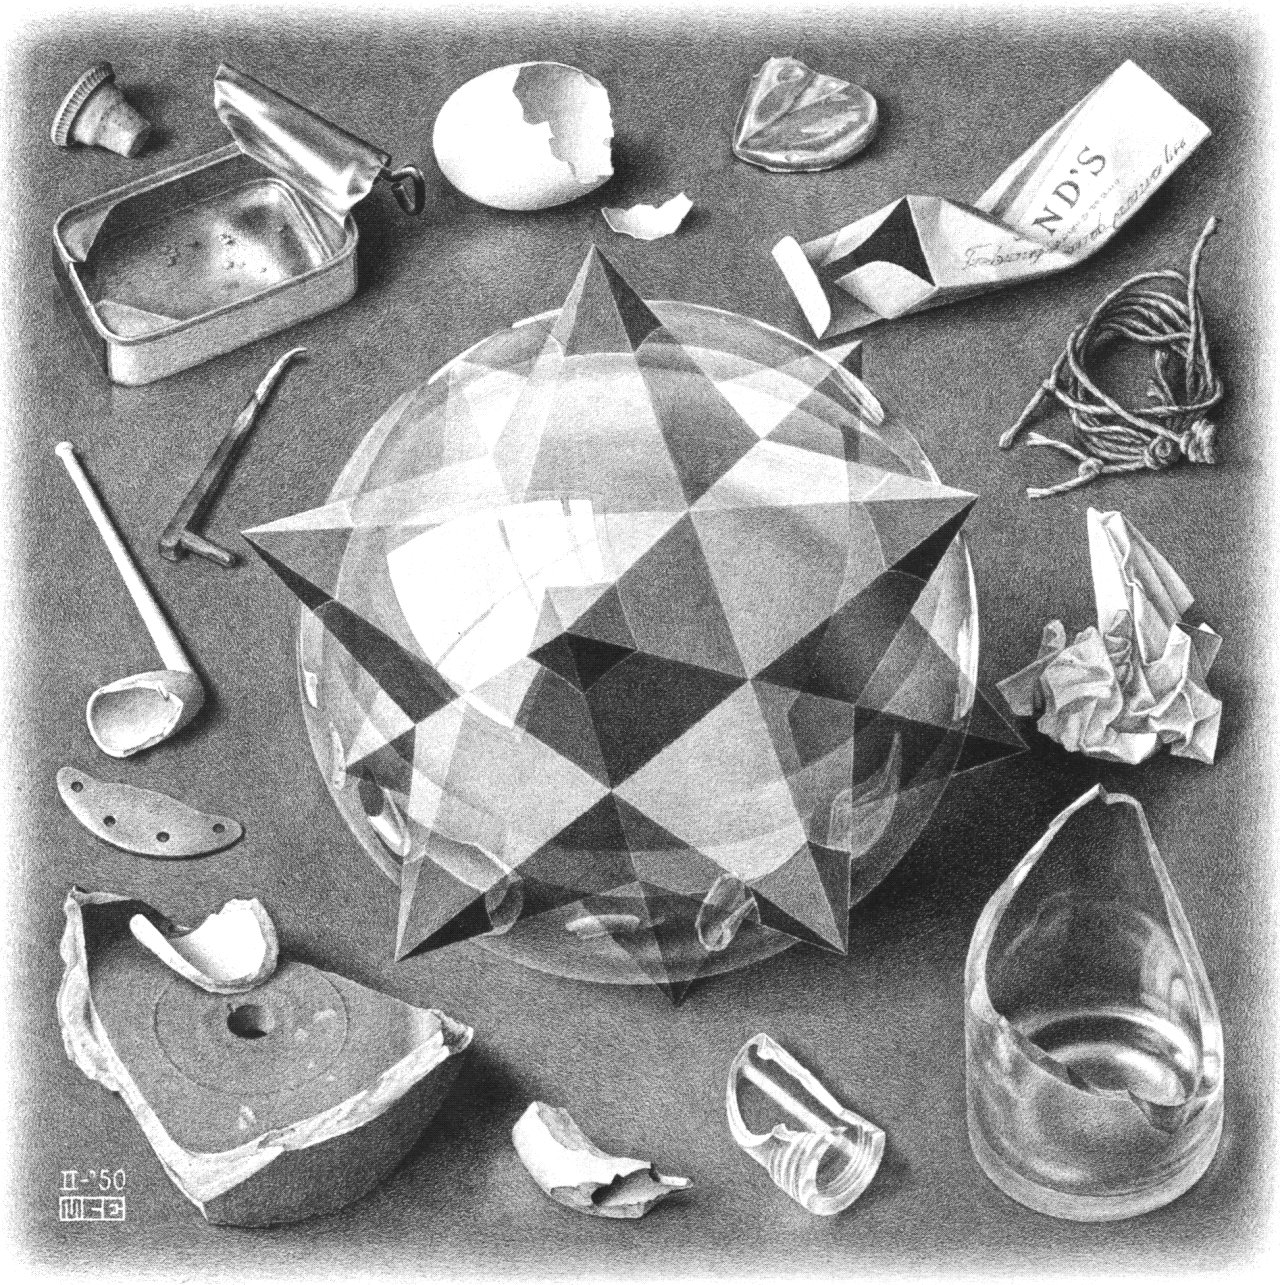
\includegraphics{img_071.jpg}
\caption[秩序与紊乱,艾舍尔作。]
  {秩序与紊乱,艾舍尔作(蚀版画,1950)。}
\end{figure}

\item[阿基里斯]“无穷巧合”?自然数中没有巧合的事——没有任何事情不是出自某种背后的规律性。不说一万亿,就说$7$吧。处理它更容易些,它比较小。$7$具有阿基里斯性质。

\item[乌龟]你肯定?

\item[阿基里斯]是的。我告诉你为什么。如果你加上$2$,就得到$9$,不是素数。如果你加上随便什么其他素数,你就是把两个奇数加在一起,结果是个偶数——这样你还是得不到一个素数。因此在这里,$7$的“阿基里斯性质”不过是——杜馔一个术语——上两条理由的“逻辑后承”,而远不是什么“无穷巧合”。这恰好支持了我的论断:说明某个算术真理时决不需要无穷步骤的推理。假若有什么算术上的事实是由无穷多的无关巧合所导致,那么你将永远无法给出一个有穷的证明。但这是荒唐的。

\item[乌龟]你这看法有些道理,而且也不止你一个人这么想。不过——

\item[阿基里斯]难道还有人不同意这个观点吗?那么这种人就必然要相信“无穷巧合”了,他们必然相信在人类创造物中最完美、最和谐、最漂亮的部分——自然数系统——当中,也有紊乱。

\item[乌龟]也许他们就是这样,可你是否想过,这种紊乱或许是美与和谐的不可分割的组成部分?

\item[阿基里斯]紊乱,完美的一部分?秩序与紊乱构成了悦人的整体?真是异端邪说!

\item[乌龟]据说你最喜欢的艺术家艾舍尔就在一幅画里暗示了这种异端观点……说起紊乱这事,我相信你会有兴趣听听两类不同的搜索,两种搜索都保证会终止。

\item[阿基里斯]当然。

\item[乌龟]第一类搜索——非紊乱型的搜索——可以用一个关于哥德巴赫性质的测试来说明。你只需看那些小于$2N$的素数,如果某一对素数加起来得到$2N$,那么$2N$就具有哥德巴赫性质,否则就不具有。这种测试不仅注定会终止,而且你还能预先知道什么时候终止。

\item[阿基里斯]那么这是个可预知其终止的测试喽。你是不是要告诉我检验某些数论性质时,要用到那种虽然保证会终止,但预先无法知道会过多久才终止的测试?

\item[乌龟]你预见得太对了,阿基,这种测试的存在就说明自然数系统从某种意义上说带有固有的紊乱。

\item[阿基里斯]这种情况下,我只好说人们还不够了解那个测试。如果他们多作些研究,他们会弄清在终止前那个测试至多要花多少时间。无论如何,整数中的模式必定是有来由的,不可能只是一些无法预知的紊乱模式!

\item[乌龟]我可以理解你这种直觉信念,阿基。不过,这一点并非总能得到证实。当然,很多情况下你是绝对正确的——仅仅因为某人不知道某事,不能得出结论说那件事不可知。可是有那么一些整数的性质,可以证明检验它们的有终测试是存在的,同时还能证明没有办法预先知道那些测试要花多少时间。

\item[阿基里斯]真难以相信。听起来就像是可恶的魔鬼阴险诡诈地溜进了自然数这属于上帝的美丽乐园!

\item[乌龟]有一点大概能安慰安慰你:想要定义出一个性质,使得能有一个有终止测试来检验它,但其终止是不可预知的,这绝不是件容易的事情,也绝不那么自然。大多数“自然的”整数性质的确都能接受可预知其终止的测试。例如:素数性、可开方性、是否是$10$的方幂等等。

\item[阿基里斯]是的,这些性质的测试全都是直截了当的。你告诉我一个那样的性质吧:检验它的唯一方法是用一个有终止测试,但不可预知其终止。

\item[乌龟]说起来太复杂了,我现在直犯困,换一个吧。我来跟你说一个很容易定义的性质,然而却还没有一个检验它的有终止测试。我没说永远不会发现这样一个测试,这一点请你注意——只是现在还没有。我们从一个数开始吧——你来选一个数。

\item[阿基里斯]$15$怎么样?

\item[乌龟]很好。我们从你这个数开始。如果它是奇数,我把它乘以$3$,再加$1$。如果它是偶数,就取其一半。然后重复这个过程。如果一个数经过这样的一些操作得到$1$,就称之为“妙极”的数,否则就称之为“非妙极”的。

\item[阿基里斯]那么$15$是妙极的还是非妙极的呢?我们看看吧。
\begin{longtable}[c]{>{$}r<{$}l<{:}>{$}r<{$}}
 15 & 是奇数,所以做$3n+1$ & 46\\
 46 & 是偶数,所以取一半 & 23\\
 23 & 是奇数,所以做$3n+1$ & 70\\
 70 & 是偶数,所以取一半 & 35\\
 35 & 是奇数,所以做$3n+1$ & 106\\
106 & 是偶数,所以取一半 & 53\\
 53 & 是奇数,所以做$3n+1$ & 160\\
160 & 是偶数,所以取一半 & 80\\
 80 & 是偶数,所以取一半 & 40\\
 40 & 是偶数,所以取一半 & 20\\
 20 & 是偶数,所以取一半 & 10\\
 10 & 是偶数,所以取一半 & 5\\
  5 & 是奇数,所以做$3n+1$ & 16\\
 16 & 是偶数,所以取一半 & 8\\
  8 & 是偶数,所以取一半 & 4\\
  4 & 是偶数,所以取一半 & 2\\
  2 & 是偶数,所以取一半 & 1
\end{longtable}

嚯!从$15$到$1$这么转弯抹角的一大圈!不过我终于还是得到$1$了。这说明$15$是具有妙极这一性质的。那么什么数会是非妙极的呢……

\item[乌龟]你注意了没有,在这么简单定义的运算下,那些数是怎样上下摆动的?

\item[阿基里斯]注意了。特别让我吃惊的是,经过十三次运算后,我得到$16$,仅比我起步时的$15$大$1$。在某种意义上说我几乎回到了出发点——而在另一种意义上,我已远离了出发点。另外还有一点使我诧异的是为了解决问题,我不得不动用大到$160$那样的一个数。我真想知道这都是为什么。

\item[乌龟]是的,有个无穷的“天空”供你飞,而且事先很难知道你会被抛到这天空里多高的地方。而且很可能你会只是不断地往高飞,越来越高,再也不下来了。

\item[阿基里斯]是吗?我猜想这倒是可能的——可这得要多奇特的巧合啊!你得正好碰上一个接一个的奇数,其中只掺有很少的几个偶数。我怀疑这到底是否会发生——可我不能肯定。

\item[乌龟]你从$27$开始怎么样?不过,我可是什么都没保证啊。有时间的话你试试,就当是玩吧。我劝你准备好一大张纸。

\item[阿基里斯]嗯……听起来挺有意思。说实在的,把妙极(或非妙极)与那个起始的数联系在一起还是让我觉得有点不安,即使很明显那是全体整数系统的性质。

\item[乌龟]我明白你的意思,“$29$是素数”,或“金子是宝贵的”这两句话没什么不同——它们都是说某一特定实体被嵌入特定语境,从而具有某一性质。

\item[阿基里斯]我想你是对的。这个“妙极”问题真是奇妙至极了,就看那些数的摆动方式吧——一会儿增大,一会儿减少。模式应该是有规则的,可是表面上却显得相当紊乱。所以我完全能想象为什么至今还没有一个检验妙极性质的有终止测试。

\item[乌龟]说起有终止过程和无终止过程,还有那些介于两者之间玩艺儿,我想起了我的一个朋友。他是个作家,正在写一本书。

\item[阿基里斯]哦?这太好了!是本什么书?

\item[乌龟]《金、银、铜——聚宝藏之精华》。挺有意思吧?

\item[阿基里斯]老实说,这名字弄得我有点糊涂了。说到底,金、银、铜之间有什么关系?

\item[乌龟]对我来说似乎是很清楚的。

\item[阿基里斯]假若书名是,比如说,“金、马、牛”,或者“风、银、牛”,嗨,我就可以把它看成……

\item[乌龟]也许你更喜欢“风、马、铜”?

\item[阿基里斯]噢,太对了!但原来那个书名太糟糕。没人能懂。

\item[乌龟]我会告诉我的朋友。他会很高兴能有一个生动易记的书名(他的出版商也会的)。

\item[阿基里斯]我真高兴。可我们的讨论怎么会让你想起他的那本书了?

\item[乌龟]啊,是这样。那本书里有篇对话,在其中他想让读者去搜索终了,从而甩掉读者。

\item[阿基里斯]竟会有这种愿望,够奇怪的。这怎么做到呢?

\item[乌龟]你无疑会注意到,一些作者在他的故事结束前的几页里如何费尽心机地建立起巨大的紧张状态——可是那个把书捧在手上的读者能感觉出故事就要结束了。所以,有某种额外的信息以一定的方式预先提醒了读者。书的物理性质多少有点破坏了那种紧张。如果,比如说,在小说的终了处有许多废话,那就会好多了。

\item[阿基里斯]废话?

\item[乌龟]对。我的意思是,有许多多余的书页,不是故事的真正组成部分,但能用来藏住终了,使得草率浏览或只凭对书的物理感觉都无法确切地得知终了在哪里。

\item[阿基里斯]我明白了。这样的话,故事的真正终了可能会出现在,比如说,书的物理终了前五十页或前一百页了?

\item[乌龟]是的。这就有了能让人兴奋的东西,因为读者事先不知道有多少页是废话,多少页是故事。

\item[阿基里斯]如果这能广为实践,会是很有效的。可是有个问题:假如这些废话非常明显——比如有许多空白,或者有充满句号或满篇杂乱无章的字词的书页,那还不如没有。

\item[乌龟]你说得对。得弄得像是正常的一页书。

\item[阿基里斯]可是一般说来即使草率地浏览正常的一页书也足以把一个故事同另一个故事区分开来。所以你必须把那些废话弄得与真正的故事非常相似。

\item[乌龟]没错。我的设想是这样:把故事讲完后不中断,继续讲下去,讲一些看上去是该故事的继续,而实际上只是些废话,与真正的主题毫无关系的事。某种意义上说,这些废话是种“终了后的终了”,带有与原主题几乎无关的多余的文学意象。

\item[阿基里斯]真够狡猾的!可这就有个问题:你无法弄清真正的终了到底在哪儿,都混在废话里了。

\item[乌龟]这也就是我的作家朋友和我所得出的结论。这是个问题,可我还是觉得那个设想相当吸引人。

\item[阿基里斯]哎,我有个建议。可以把从真正的故事到废话部分的转折做成这样:一个有智能的阅读者对正文充分专注仔细地审查之后,能查明什么地方是前者的结束、后者的开始。也许这会使他花费相当的时间。也许没有办法预先知道到底要花多长时间……但出版者能够保证对真正终了的一个充分专注仔细的搜索一定会终止,即使他无法在其终止前说出到底要花多少时间。

\item[乌龟]很好——但“充分专注仔细”是什么意思?

\item[阿基里斯]意思是:读者必须专注地寻找出现在正文某处的某种微小、然而却说明问题的特征。那特征标志着终了。他还必须有足够的聪明去思考并搜寻许多这类特征,直到发现了真正标志终了的那个特征。

\item[乌龟]比如说某些字的出现频率的突然变化,或一些成语的一部分被莫名其妙地丢掉了,或者突然涌现出一连串语法错误?

\item[阿基里斯]可能是吧。或者是某种隐藏着的信息,对于一个充分专注仔细的读者,它会揭示出真正的终了。你甚至还可以加进一些额外的角色或事件,它们与前面故事的精神很不协调。一个头脑简单的读者会囫囵吞枣地一直把书读完,而有头脑的读者就能够准确地找到分界线在哪里。

\item[乌龟]这真是个有独创性的想法,阿基。我会电告我的朋友,说不定他在他的对话里就用上你这方法了。

\item[阿基里斯]我不胜荣幸。

\item[乌龟]好啦,阿基,我得回去了。我恐怕都有点站不稳了,趁现在还能找着路,我最好现在就走。

\item[阿基里斯]你为了我而在这儿待了这么长时间,而且是在夜里的这种时候,真让我受宠若惊。我敢保证你那数论娱乐对于我的辗转不眠是绝好的良方。真的——没准我今晚能睡个好觉了。龟兄,我愿送给你一件特别的礼物,以表我的感激之情。

\item[乌龟]噢,别这样,阿基。

\item[阿基里斯]这是我的一点心意,龟兄。到柜子那儿去,你会在上面找一个金色的小包。

\dnote{(乌龟慢吞吞地踱到阿基里斯的柜子前。)}

\item[乌龟]你不是指这个人造革的包吧?

\item[阿基里斯]就是那个。不过那不是人造革的,它是变造革的。

\item[乌龟]什么是变奏歌?

\item[阿基里斯]哦,你听岔了,不是什么“变奏歌”,我是说“变造革”,这是种金、银、铜的聚合物,看上去像皮子。请收下吧,龟兄,作为我最衷心的祝愿。

\item[乌龟]的确太谢谢你啦,阿基,嗯……哎,这包上面印的是什么呀?哦,是英文呐,多古怪的一份名单啊:
\begin{center}
\setlength\tabcolsep{1pt}
\begin{tabular}{*{11}c}
\emph{D}&e&&M&o&r&g&a&n\\
A&\emph{b}&e&l\\
B&o&\emph{o}&l&e\\
B&r&o&\emph{u}&w&e&r\\
S&i&e&r&\emph{p}&i&n&s&k&i\\
W&e&i&e&r&\emph{s}&t&r&a&s&s
\end{tabular}
\end{center}
\item[阿基里斯]我相信这一定是一份完整的所有伟大数学家的名单。

\item[乌龟]真的吗?我看看——德·摩根、阿贝尔、布尔、布劳维、谢尔平斯基、维尔斯特拉斯——哦,没错,他们确实全都是世界著名的数学家。可这名单上怎么没有康托尔的名字?让我瞧瞧,我想他的名字的拼法是“Cantor”。

\item[阿基里斯]我真想象不出他的名字怎么能不包括在内。我也弄不明白为什么对角线上的那些字母用了黑体。

\item[乌龟]下面写着:“从该对角线中减$1$,就能找到巴赫在莱比锡的职位”。

\item[阿基里斯]我也看到了,可我完全不知所云,哎,喝上两口上好的威士忌怎么样?我架子上的那只瓶子里正好有点儿。

\item[乌龟]不必啦。我已经累坏了。我得赶紧回去了。\dlnote{(他漫不经心地打开了小包。)}哎,等等,阿基——这里面装的是一百枚金币!

\item[阿基里斯]你要是能收下,我将非常非常高兴,龟兄。

\item[乌龟]可是——可是——

\item[阿基里斯]别再客气了。那小包,那金子——都是你的了。为这个无与伦比的晚上,我衷心地感谢你。好了,再见吧,龟兄。

\item[乌龟]我没能做到善始善终,我本想帮你克服失眠症,可现在只好无功受禄、不了了之。好吧,谢谢你的礼物,再见。

\dnote{(这时,传来什么人的敲门声。)}

都这么晚了,谁还会来敲门?

\item[阿基里斯]我一点儿也想不出来会是谁。我觉得多少有点问题。你还是躲到柜子后面去吧,免得碰上什么麻烦事。

\item[乌龟]好主意。\dlnote{(费力地挤到柜子后面。)}

\item[阿基里斯]谁啊?

\item[声音]开门!我们是警察!

\item[阿基里斯]请进,门开着呢。

\dnote{(两个粗壮的警察推门进来,身上带着闪亮的徽章。)}

\item[警察]\dlnote{(指着自己的铜徽章)}我姓银。他姓金。这里是不是住着一个叫阿基里斯的?

\item[阿基里斯]我就是。

\item[警察]那好,阿基里斯,我们有理由相信有一个变造革的包在这儿,里面有一百枚金币。今天下午有人在博物馆里把它弄到手后溜走了。

\item[阿基里斯]哎哟我的老天!

\item[警察]如果是这儿,阿基里斯,由于你是唯一可能的嫌疑,很遗憾我必须拘留你。我带来了搜查证——

\item[阿基里斯]噢。先生们,你们来我真高兴!我被乌龟先生还有他那个变造革的包吓得一晚上都不自在。现在你们终于来了,这下我可得救了!快,先生们,就在那柜子后面,罪犯就在那里!\dlnote{(警察往柜子后面看去,看见乌龟在里面缩成一团,抱着他那变造革的包,浑身打颤。)}

\item[警察]就在这儿!那么乌龟先生就是那个混蛋喽,嗯?我可没想到是他!可是他被当场抓住了!

\item[阿基里斯]把这恶棍带走,好心的先生们!谢天谢地,这可将是我最后一次见他和那个变造革的包了!

\end{dialogue}

\end{dialog}
